%------------------------------------------- Sample ------------------------------------

%% \lipsum[81-100]
%
%\begin{figure}
%  \centering
%  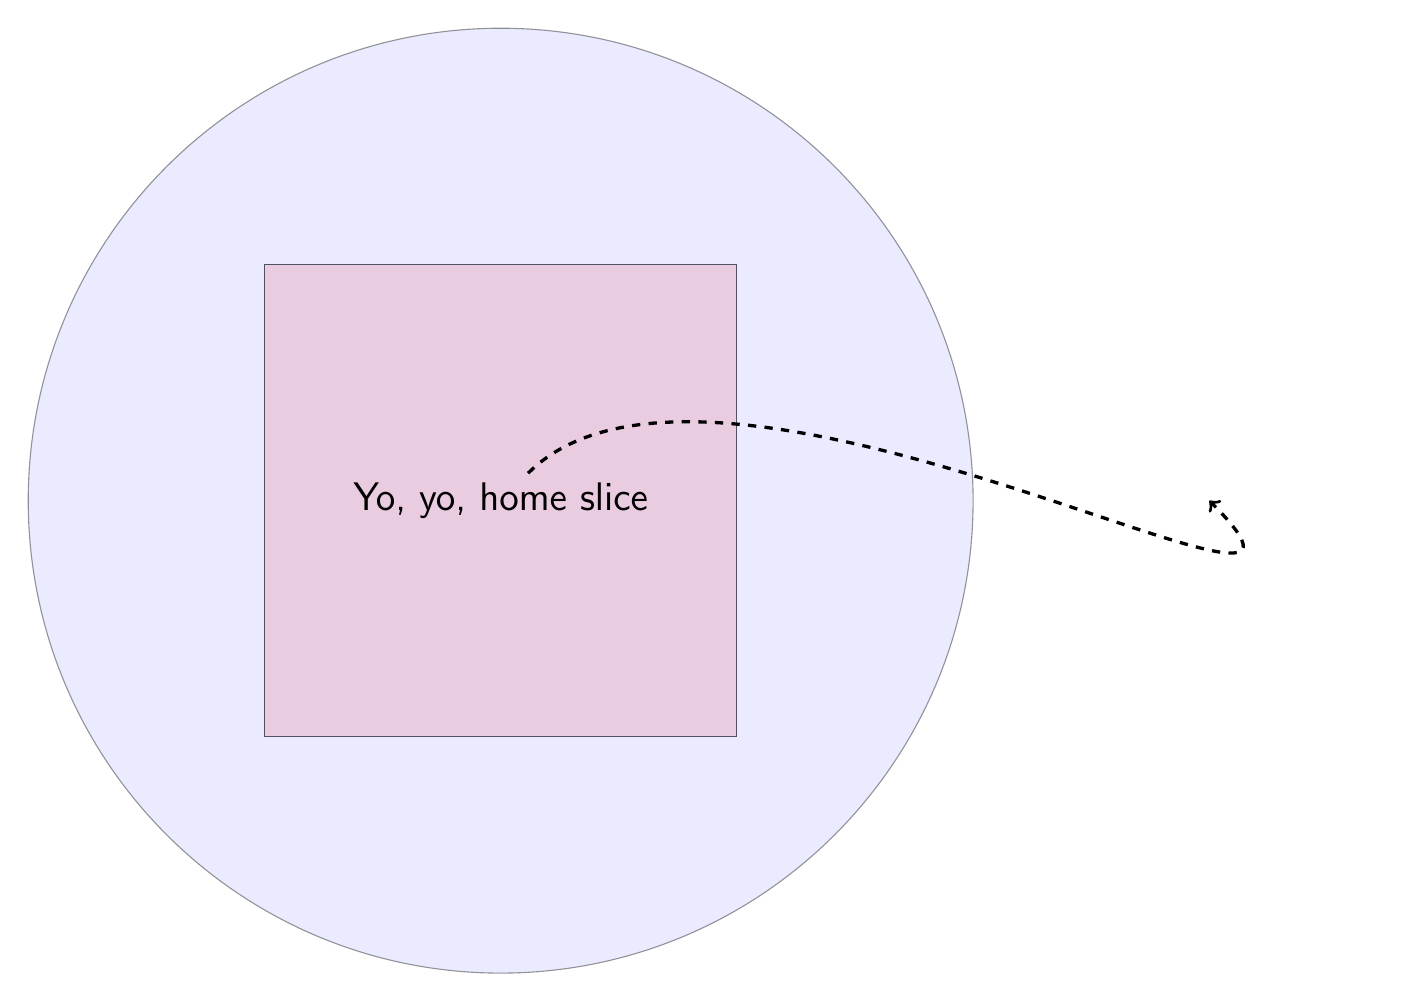
\begin{tikzpicture}[scale=3]

  \draw [fill=red!20!white] (1,1) -- ++(0,-2) -- ++(-2,0) -- ++(0,2) -- cycle;
  \draw [fill=blue!20!white,opacity=0.4] (0,0) circle(2cm);
  \node [font={\Large\sf}] (yo) at (0,0) {Yo, yo, home slice};
  \draw[->,very thick, dashed] (yo) to [out=45,in=-45] (3,0);

\end{tikzpicture}

%  \caption[Awesome picture]{Isn't this picture awesome?}
%\end{figure}
%
%\begin{figure}
%  \centering
%  \begin{tikzpicture}
  \draw [fill=red!70!white,circular drop shadow={shadow scale=1.05},very
  thick,rotate=45,opacity=0.7] (0,0) rectangle (3,2);


  \draw [fill=blue!70!white,circular drop shadow={shadow scale=1.05},very
  thick,rotate=135,opacity=0.7] (0,0) rectangle (3,2);
  \draw [fill=orange!70!white,circular drop shadow={shadow scale=1.05},very
  thick,rotate=225,opacity=0.7] (0,0) rectangle (3,2);
  \draw [fill=green!70!white,circular drop shadow={shadow scale=1.05},very
  thick,rotate=-45,opacity=0.7] (0,0) rectangle (3,2);
\end{tikzpicture}

%  \caption[Tubular picture]{Totally tubular, dude}
%\end{figure}

%------------------------------------------- Real ----------------------------------------

In this chapter, we are going to describe the numerical scheme for solving the coupled system of equations in both boundary layer and the outer region, i.e, how to evolve the quantity from time step $n$ to time step $n+1$.


\section{Outer flow}
In the outer region, the inviscid equation (???) is integrated using vortex methods, which are based on the discretization of vorticity field and the Lagrangian description of governing equations (???) and (???) that, when solved, determine the evolution of the computational elements.
As usual, vortex methods enjoy advantages such as the use of computational elements only in regions with nonzero vorticity, the automatic adaptivity of the computational elements, and the rigorous treatment of boundary conditions at infinity.
Besides, we only need the flow velocity on $C$ , which is decomposed into rotational part and potential part as
\begin{align}
\bu^n &  = (\bu_{\omega o} + \bu_{\omega n_-} + \grad \phi)^n, \\
\bu^{n+1} & = (\bu_{\omega o}+ \bu_{\omega n_+} + \grad \phi)^{n+1}.
\end{align}
As before, $\bu_{\omega o}$ is velocity induced by vortices which are in the outer region at both time steps $n$ and $n+1$, $\bu_{\omega n_-}$ is by those which are in outer region at time $n$ but enter boundary layer through $C$ in step $n+1$, $\bu_{\omega n_+}$ is on the contrary by those which are added to outer region due to outward vorticity flux across $C$.
Accordingly, the $\theta$-component of (???) and (???) can be discretized as
\begin{align} \label{eqn:Eulersplit}
\frac{u_{\omega o}^{n+1}-u_{\omega o}^{n} }{\Delta t} +  [\frac{|\bu|^2}{2}]^n_{,\theta}  =   -p_{\omega,\theta}^{n+1},  \quad
\frac{{\phi}_{,\theta}^{n+1}-{\phi}_{,\theta}^{n} }{\Delta t}  =   -p_{\phi,\theta}^{n+1}
\end{align}
The rotational part $\bu_{\omega o}^{n+1}$ can be calculated through advecting vortices by local fluid velocity $\frac{d\bx}{dt} = \bu(\bx)$ and then evaluating the velocity by vortices at new locations using Biot-Savart law (???).
Fast multipole method (see next subsection) can be used to reduce the cost of evaluating pairwise interactions between $N$ vortices to order $N\ln N$ from $N^2$ which is the cost by direct summation.
If necessary, vortices which get close to each other and far from the body can be merged since their influences on the flow around body are weak.
By this, the total number of vortices $N$ which needs to be tracked can be well controlled, which is useful for long-term simulation.
With $\bu_{\omega o}^{n+1}$, the first equation of (???) gives $p_{\omega,\theta}^{n+1}$.
Vorticity flux across $C$ corresponds to vortex shedding (outward flux) or vortex recapture (inward flux), and mathematically they are represented as (???), or discretely
\begin{align} \label{eqn:vorticityflux}
-\frac{u_{\omega n_-}^n}{\Delta t} + [v_- \omega]_{\eta_m}^n = 0, \quad
\frac{u_{\omega n_+}^{n+1}}{\Delta t} + [v_+ \omega]_{\eta_m}^n = 0.
\end{align}
The shedding of new vortices into outer region has to be in such a way that the velocity induced by them is exactly $u_{\omega n_+}^{n+1}$.

\subsection{Lagrangian description}

\subsection{Fast vortex methods}
The straightforward method of computing the velocity induced by every particle requires O($N^2$) operations for $N$ vortex elements.
This precludes high-resolution studies of bluff body flows with more than say 50000 elements.
However, fast methods exist that have operation counts of O($N\log N$)  (Barnes \& Hut 1986) or O($N$) (Greengard \& Rocklin 1987) depending on the details of the algorithm.
The basic idea of these methods is to decompose the element population spatially into clusters of particles and build a hierarchy of clusters or a 'tree' - smaller neighboring clusters combine to form a cluster of the next size up in the hierarchy and so on.

The contribution of a cluster of particles to the velocity of a given vortex can then be computed to desired accuracy if the particle is sufficiently far from the cluster in proportion to the size of the cluster and a sufficiently large number of terms in the multipole expansion is taken.
This is the essence of the 'particle-box' method, requiring O($N\log N$) operations.
One then tries to minimize the work required by maximizing the size of the cluster used while keeping the number of terms in the expansion within a reasonable limit and maintaining a certain degree of accuracy.

The 'box-box' scheme goes one step further as accounts for box-box interactions as well. 
These interactions are in the form of shifting the expansions of a certain cluster with the desired accuracy to the center of another cluster.
Then those expansions are used to determine the velocities of the particles in the second cluster.
This has the effect of minimizing the tree traversals for the individual particles, requiring only $O(N)$ operations.
In our numerical implementation, this scheme is utilized.

\section{Inner flow}

In order to match with the outer flow, boundary layer flow is similarly decomposed into two parts as $\bu = \bu_a + \bu_b$.
$\bu_a$ matches with $\bu_\omega$ at $C$ and satisfies
\begin{align} \label{eqn:ua}
\frac{u_a^{n+1}-(u^n-u_\phi^n) }{\Delta t}  + [\frac{|\bu|^2}{2}]^n_{,\theta} + (v \omega)^n
 =   -p^{n+1}_{\omega,\theta} + \visc u^{n+1}_{a,\eta\eta}
\end{align}
and the boundary conditions
\begin{align} \label{eqn:uaBC}
u_a^{n+1}(\eta_0) = 0, \quad u_a^{n+1}(\eta_m) = u_\omega^{n+1}.
\end{align}
(???) and (???) are complete to calculate $u_a^{n+1}$ with $p_{\omega, \theta}^{n+1}$ given by (???), and then $v_a^{n+1}$ can be calculated by incompressible condition.
The other part $\bu_b$ matches with $\bu_\phi$ and satisfies
\begin{align} \label{eqn:ub}
\frac{u_b^{n+1}- u_\phi^n }{\Delta t} =   -p^{n+1}_{\phi,\theta} + \visc u^{n+1}_{b,\eta\eta}
\end{align}
and the boundary conditions
\begin{align} \label{eqn:ubBC}
u_a^{n+1}(\eta_0) = 0, \quad u_a^{n+1}(\eta_m) = u_\phi^{n+1}.
\end{align}
Combined with (???), the equation can be solved analytically as  $u_b^{n+1} = u_{\phi}^{n+1}(\theta) [1- u_h(\eta)] $ with $u_h = \sinh[(\eta_m - \eta)/\sqrt{\visc \Delta t}] / \sinh[(\eta_m - \eta_0)/\sqrt{\visc \Delta t}]$. Then by continuity equation, the normal component is $v_b^{n+1} = -Q u_{\phi,\theta}^{n+1}$ with $Q = \int_{\eta_0}^{\eta} d\eta [1 - u_h(\eta)]$.


\section{Coupling}

With $\bu_\omega^{n+1}$ and $\bu_a^{n+1}$ already calculated, the remaining unknown is the potential flow $\bu_{\phi}^{n+1}$. 
It can be solved as follows by matching the normal velocity of boundary layer and outer region at $C$.
From the outer region, the total normal velocity at $C$ is $v^{n+1} = v_\omega^{n+1} + v_\phi^{n+1}$.
In the boundary layer, the total normal velocity on $C$ can be written as $v^{n+1} = [u_a^{n+1} + v_b^{n+1}]_{\eta_m}  = [ v_a^{n+1}  - Q u_{\phi, \theta}^{n+1}]_{\eta_m}$.
So the matching of $v^{n+1}$ gives the condition for potential flow
\begin{align} \label{eqn:matching}
Q u_{\phi, \theta}^{n+1} + v_{\phi}^{n+1} = v_a^{n+1} - v_\omega^{n+1} \quad \text{on~} C.
\end{align}
(???) together with the condition at $\infty$ provides enough conditions for (???). In general, boundary integral method gives the solution.
Depending on the shape of $C$, faster method may be possible.

\subsection{Analytical Solution for Circular Geometry}

In the special case of circular geometry, equation (???) can be solved analytically as follows. 
The general solution of Laplacian equation outside a circle with uniform flow at infinity is
 \begin{eqnarray} 
\phi_{nc} = Ur\cos\theta + \frac{1}{2\pi}(m\ln r + \kappa \theta)
+ \sum_{n=1}^{\infty} \frac{A_n e^{in\theta}+c.c. }{r^n}
\end{eqnarray}
with the velocity field
 \begin{eqnarray} 
u_{nc} & = & \frac{1}{r} \frac{\partial \phi_{nc}}{\partial \theta}  =  -U\sin\theta + \frac{\kappa}{2\pi r}
+ \sum_{n=1}^{\infty} \frac{ in (A_n e^{in\theta}-c.c.) }{r^{n+1}} \\
v_{nc} & = & \frac{\partial \phi_{nc}}{\partial r}  =   U\cos\theta + \frac{m}{2\pi r}
+ \sum_{n=1}^{\infty} \frac{ -n (A_n e^{in\theta}+c.c.) }{r^{n+1}}
\end{eqnarray}
Then equation (\ref{eqn:potential}) becomes
 \begin{eqnarray} 
\frac{m}{2\pi c} + \sum_{n=1}^{\infty} \frac{ (-n-n^2Q) (A_n e^{in\theta}+c.c.) }{c^{n+1}}
= F + (Q-1)U\cos \theta
\end{eqnarray}
with the solution
\begin{eqnarray} 
m = 2 \pi c \hat{F}_0,  & & A_n = -\frac{c^{n+1}}{n+n^2Q} \hat{F}_n + \frac{Uc^2(1-Q)}{2(1+Q)} \delta_{n1}
\end{eqnarray}
where $\hat{F}_n$ is the Fourier  coefficient of $F(\theta)$.

\subsection{Boundary Integral Method}

